\documentclass[11pt]{article}
\usepackage[a4paper,margin=22mm]{geometry}
\usepackage[no-math]{fontspec}
\setmainfont{lmroman10-regular.otf}[BoldFont=lmroman10-bold.otf,ItalicFont=lmroman10-italic.otf,BoldItalicFont=lmroman10-bolditalic.otf]
\usepackage{amsmath,amssymb,amsthm,mathtools,graphicx,xcolor,hyperref,xurl,xspace,ifthen}
\setlength{\emergencystretch}{4em}
\SetMathAlphabet{\mathbf}{normal}{OT1}{cmr}{bx}{n}
\SetMathAlphabet{\mathbf}{bold}{OT1}{cmr}{bx}{n}
\newtheorem{theo}{Theorem}[section]
\newtheorem{lemm}[theo]{Lemma}
\newtheorem{theorem}[theo]{Theorem}
\newtheorem*{remas*}{Remarks}
\newtheorem{remas}[theo]{Remarks}
\newtheorem*{exam*}{Example}
\newtheorem{ques}[theo]{Question}
\providecommand{\og}{«\nobreakspace}
\providecommand{\fg}{\nobreakspace»}
\newtheorem{lem}[theo]{Lemma}
\newtheorem{lemma}[theo]{Lemma}
\newtheorem{prop}[theo]{Proposition}
\newtheorem{coro}[theo]{Corollary}
\newtheorem{corol}[theo]{Corollary}
\newtheorem{conj}[theo]{Conjecture}
\newtheorem{Proposition}[theo]{Proposition}
\newtheorem{theoreme}[theo]{Theorem}
\theoremstyle{definition}
\newtheorem{defi}[theo]{Definition}
\newtheorem{exam}[theo]{Example}
\newtheorem{exem}[theo]{Example}
\newtheorem{rema}[theo]{Remark}
\newtheorem{nota}[theo]{Notation}
\newtheorem*{rema*}{Remark}
\newtheorem*{defi*}{Definition}
\newtheorem*{theo*}{Theorem}
\newtheorem*{lemm*}{Lemma}
\newtheorem*{prop*}{Proposition}
\newcommand{\enoncename}{}
\newtheorem{corpusenonce}[theo]{\enoncename}
\newenvironment{enonce}[2][]{\renewcommand{\enoncename}{#2}\begin{corpusenonce}}{\end{corpusenonce}}
\newenvironment{enonce*}[2][]{\par\medskip\noindent\textbf{#2.}\itshape}{\par\medskip}
\newenvironment{proofc}[1][\proofname]{\begin{proof}[#1]}{\end{proof}}
\newcommand{\Mc}{\mathcal{M}}
\newcommand{\pointir}{.\ ---\ }
\providecommand{\mathof}[1]{\mathrm{#1}}

\numberwithin{equation}{section}
\numberwithin{figure}{section}
\numberwithin{table}{section}
\def\endappendix{}
%~Mouliné par MaN_auto v.0.21.6 2019-08-21 16:45:33


\usepackage{amssymb}

\DeclareMathOperator{\cov}{cov}
\DeclareMathOperator{\Var}{Var}








\newcommand{\1}[1]{{\mathbf 1}{\{#1\}}}
\newcommand{\eps}{\varepsilon}
\newcommand{\Z}{\mathbb{Z}}
\newcommand{\V}{{\mathcal V}}
\newcommand{\RR}{{\mathcal R}}
\newcommand{\R}{{\mathbb R}}
\newcommand{\Ex}{{\mathcal{E}\!\!\text{\footnotesize{\textsl{x}}}}}
\newcommand{\s}{{\widehat S}}
\newcommand{\hN}{{\widehat N}}
\newcommand{\FFF}{{\mathcal F}}
\newcommand{\8}{{\infty}}
\newcommand{\hh}{{\bar h}}
\newcommand{\hq}{{\bar q}}
\newcommand{\IP}{{\mathbb P}}
\newcommand{\IE}{{\mathbb E}}
\newcommand{\hP}{\widehat{P}}
\newcommand{\hH}{{\widehat H}}
\newcommand{\htau}{\widehat{\tau}}
\newcommand{\B}{{\mathsf B}}

%\allowdisplaybreaks

\graphicspath{{./figures/}}

\newcommand*{\mk}{\mkern -1mu}
\newcommand*{\Mk}{\mkern -2mu}
\newcommand*{\mK}{\mkern 1mu}
\newcommand*{\MK}{\mkern 2mu}

\hypersetup{urlcolor=purple, linkcolor=blue, citecolor=red}

\newcommand*{\romanenumi}{\renewcommand*{\theenumi}{\roman{enumi}}}
\newcommand*{\Romanenumi}{\renewcommand*{\theenumi}{\Roman{enumi}}}
\newcommand*{\alphenumi}{\renewcommand*{\theenumi}{\alph{enumi}}}
\newcommand*{\Alphenumi}{\renewcommand*{\theenumi}{\Alph{enumi}}}


\begin{document}
\section*{\raggedright 2689: Uniform limiting visited fraction in dilated bounded open planar sets for simple random walk conditioned to avoid the origin}
\noindent\textbf{Author:} Nina Gantert; Serguei Popov; Marina Vachkovskaia\par\noindent\textbf{Source:} On the range of a two-dimensional conditioned simple random walk. Annales Henri Lebesgue 2 (2019), publisher version, DOI 10.5802/ahl.20. \url{https://ahl.centre-mersenne.org/item/AHL_2019__2__349_0/}
\par\noindent\textbf{License:} CC BY 4.0, \url{https://creativecommons.org/licenses/by/4.0/}. The original publisher PDF has the explicit license notice. See the saved source/license records.
\par\noindent\textbf{Editorial material note (not author text):} The selected problem is Corollary 1.3: the Uniform[0,1] distributional limiting visited and unvisited proportions in dilates of a nonempty bounded open planar set, for the potential-kernel Doob walk avoiding zero and started at a fixed neighbour of zero. The complete author body retains the local hitting probabilities, geometric mesoscopic-excursion count, spatial covariance/variance, fixed-s bracketing and corollary inner-ball deletion. Three original graphical illustrations remain figure-only assets with native editable captions. Quantitative Kolmogorov bounds and hole/recurrence/Liouville assertions are unselected context; named potential-kernel and conditioned-walk prerequisites remain references. All proof text and formulas below are editable author TeX. Mathematical wording, language and proof order are retained. Only the article class, title matter and bibliography presentation are adapted for independent compilation; no proof has been generated or repaired.
\par\noindent\textbf{Editorial difficulty:} H2: The proof isolates a geometric number of mesoscopic excursions and separates its randomness from correlated spatial coverage through potential-kernel hitting bounds and covariance estimates. The uniform range-fraction law for a transient conditioned walk exceeds ordinary qualifying probability.
\par\noindent\textbf{Editorial retrieval and attribution:} Retrieved 2026-10-01. DOI 10.5802/ahl.20. Source attribution notice: ../licenses/2689-source-license.txt; complete legal text: ../licenses/CC-BY-4.0.txt. Original source excerpts and the existing source-material check are retained in ../sources/2689/.
\medskip\hrule\medskip
\noindent\textbf{Author statement, complete proof and local supporting text follow in source order.}
\section{Introduction and results}\label{s_introres}

We start by introducing some basic notation and defining the ``conditioned'' random walk~$\s$, the main object of study in this paper. Besides being interesting on its own, this random walk is the main ingredient in the construction of the two-dimensional random interlacements of~\cite{CP16,CPV16} (see also~\cite{CT12,DRS14,SLT,Szn10} for the higher-dimensional case).

Write~$x\sim y$ if $x$ and $y$ are neighbours in~$\Z^2$. Let~$(S_n, n\geq 0)$ be two-dimensional simple random walk, i.e., the discrete-time Markov chain with state space~$\Z^2$ and transition probabilities defined in the following way:
\begin{equation}\label{def_S}
P_{xy} =
\begin{cases}
\dfrac{1}{4}, & \text{if }x\sim y,\\[0.6em]
0, & \text{otherwise}.
\end{cases}
\end{equation}
We assume that all random variables in this paper are constructed on a common probability space with probability measure~$\IP$ and we denote by~$\IE$ the corresponding expectation. When no confusion can arise, we will write~$\IP_x$ and~$\IE_x$ for the law and expectation of the\footnote{The simple one, or the conditioned one defined below.} random walk started from~$x$. Let
\begin{align}
\tau_0(A) &= \inf\{k\geq 0: S_k\in A\} \label{entrance_t},\\
\tau_1(A) &= \inf\{k\geq 1: S_k\in A\} \label{hitting_t}
\end{align}
be the entrance and the hitting time of the set~$A$ by simple random walk~$S$ (we use the convention $\inf \emptyset = +\8$). For a singleton $A=\{x\}$, we will write $\tau_i(A)=\tau_i(x)$, $i=0,1$, for short. One of the key objects needed to understand the two-dimensional simple random walk is the potential kernel~$a$, defined by
\begin{equation}\label{def_a(x)}
a(x) = \sum_{k=0}^\infty\big(\IP_0[S_k\!=\!0]-\IP_x[S_k\!=\!0]\big).
\end{equation}
It can be shown that the above series indeed converges and we have~$a(0)=0$, $a(x)>0$ for $x\neq 0$. It is straightforward to check that the function~$a$ is harmonic outside the origin, i.e.,
\begin{equation}\label{a_harm}
\frac{1}{4}\sum_{y: y\sim x}a(y) = a(x) \quad \text{ for all } x\neq 0.
\end{equation}
Also, using~\eqref{def_a(x)} and the Markov property, one can easily obtain that $\frac{1}{4}\sum_{x\sim 0}a(x)=1$, which implies by symmetry that
\begin{equation}\label{a(x)=1}
a(x)=1 \text{ for all }x\sim 0.
\end{equation}

Observe that~\eqref{a_harm} immediately implies that $a(S_{k\wedge \tau_0(0)})$ is a martingale, we will repeatedly use this fact in the sequel. Further, one can show that (with $\gamma=0.5772156\dots$ the Euler--Mascheroni constant)
\begin{equation}\label{formula_for_a}
a(x) = \frac{2}{\pi}\ln \|x\| + \frac{2\gamma+ 3\ln 2}{\pi} + O(\|x\|^{-2})
\end{equation}
as $x\to\infty$, cf.~\cite[Theorem~4.4.4]{LL10}.

Let us define another random walk $(\s_n, n\geq 0)$ on~$\Z^2\setminus \{0\}$ in the following way: its transition probability matrix equals (compare to~\eqref{def_S})
\begin{equation}\label{def_hatS}
\hP_{xy} =
\begin{cases}
\displaystyle\frac{a(y)}{4a(x)}, & \text{ if } x\sim y, x\neq 0,\\
0,\phantom{\int\limits^A} & \text{ otherwise.}
\end{cases}
\end{equation}
It is immediate to see from~\eqref{a_harm} that the random walk~$\s$ is indeed well defined.

The walk~$\s$ is the Doob $h$-transform of the simple random walk, under the condition of not hitting the origin (see~\cite[Lemma~3.3 and its proof]{CPV16}). Let $\htau_0, \htau_1$ be defined as in~\eqref{entrance_t}--\eqref{hitting_t}, but with~$\s$ in the place of~$S$. We summarize the basic properties of the walk~$\s$ in the following

\begin{prop}\label{p_basic_prop}
The following statements hold:
\begin{enumerate}
\item \label{1.1.1} The walk~$\s$ is reversible, with the reversible measure~$\mu_x:=a^2(x)$.
\item \label{1.1.2} In fact, it can be represented as a random walk on the two-dimensional lattice with conductances $\big(a(x)a(y), x,y\in \Z^2, x\sim y\big)$.
\item \label{1.1.3} Let~$\mathcal{N}$ be the set of the four neighbours of the origin. Then the process $1/a(\s_{n\wedge \htau_0(\mathcal{N})})$ is a martingale.
\item \label{1.1.4} The walk $\s$ is transient.
\item \label{1.1.5} Moreover, for all $x\neq 0$
\begin{equation}\label{escape_from_site}
\IP_x\big[\htau_1(x)<\infty\big] = 1-\frac{1}{2a(x)},
\end{equation}
and for all $x\neq y$, $x,y\neq 0$
\begin{equation}\label{not_hit_site}
\IP_x\big[\htau_0(y)<\infty\big] =
\IP_x\big[\htau_1(y)<\infty\big] = \frac{a(x)+a(y)-a(x-y)}{2a(x)}.
\end{equation}
\end{enumerate}
\end{prop}

The statements of Proposition~\ref{p_basic_prop} are not novel (they appear already in~\cite{CPV16}), but we found it useful to collect them here for the sake of completeness and also for future reference. We will prove Proposition~\ref{p_basic_prop} in the next section. It is curious to observe that~\eqref{not_hit_site} implies that, for any~$x$, $\IP_x[\htau_1(y)<\infty]$ converges to $\frac{1}{2}$ as $y\to \infty$. As noted in~\cite{CPV16}, this is related to the remarkable fact that if one conditions on a very distant site being vacant, then this reduces the intensity ``near the origin'' of the two-dimensional random interlacement process by a factor of four.

Let~$\|{\,\cdot\,}\|$ be the Euclidean norm. Define the (discrete) ball
\[
\B(x,r) = \{y\in \Z^2: \|y-x\|\leq r\}
\]
(note that this definition works for \emph{all} $x\in\R^2$ and $r\in\R_+$), and abbreviate $\B(r):=\B(0,r)$. The (internal) boundary of $A\subset\Z^2$ is defined by
\[
\partial A = \{x\in A: \text{there exists }y\in \Z^2\setminus A
\text{ such that }x\sim y\}.
\]

Now we introduce some more notation and state the main results. For a set $T\subset\Z_+$ (thought of as a set of time moments) let
\[
\s_T=\bigcup_{m\in T}\big\{\s_m\big\}
\]
be the \emph{range} of the walk~$\s$ with respect to that set. For simplicity, we assume in the following that the walk~$\s$ starts at a fixed neighbour~$x_0$ of the origin, and we write $\IP$ for $\IP_{x_0}$ (it is, however, clear that our results hold for any fixed starting position of the walk). For a nonempty and finite set $A\subset \Z^2$, let us consider random variables
\begin{align*}
\RR(A) &= \frac{\big|A\cap \s_{[0,\infty)}\big|}{|A|},\\
\V(A) &= \frac{\big|A\setminus \s_{[0,\infty)}\big|}{|A|} = 1-\RR(A);
\end{align*}
that is, $\RR(A)$ (respectively, $\V(A)$) is the proportion of visited (respectively, unvisited) sites of~$A$ by the walk~$\s$. Let us also abbreviate, for $M_0 > 0$,
\begin{equation}\label{df_ell_A}
\ell^{(n)}_A= |A|^{-1}
\max_{y\in A}
\big|A\cap \B\big(y,{\tfrac{n}{\ln^{M_0}n}}\big)\big|.
\end{equation}
Our main result is the following
\begin{theo}\label{t_main_res}
Let $M_0>0$ be a fixed constant, and assume that $A\subset \B(n)\setminus \B(n\ln^{-M_0}n)$. Then, for all $s\in [0,1]$, we have, with positive constants $c_{1,2}$ depending only on~$M_0$,
\begin{equation}\label{main_res}
\big|\IP[\V(A)\leq s] - s\big|
\leq c_1\Big(\frac{\ln\ln n}{\ln n}\Big)^{1/3} + c_2\ell^{(n)}_A \Big(\frac{\ln\ln n}{\ln n}\Big)^{-2/3},
\end{equation}
and the same result holds with~$\RR$ on the place of~$\V$.
\end{theo}

The above result means that if~$A\subset \B(n)\setminus \B(n\ln^{-M_0}n)$ is ``big enough and well distributed'', then the proportion of visited sites has approximately Uniform$[0,1]$ distribution. In particular, one can obtain the following

\begin{coro}\label{cor_open}
Assume that $D\subset \R^2$ is a bounded open set. Then both sequences $(\RR(nD\cap\Z^2),n\geq 1)$ and $(\V(nD\cap\Z^2),n\geq 1)$ converge in distribution to the Uniform$[0,1]$ random variable.
\end{coro}

Indeed, it is straightforward to obtain it from Theorem~\ref{t_main_res} since $|nD\cap\Z^2|$ is of order $n^2$ as $n\to\infty$ (note that~$D$ contains a disk), and so $\ell^{(n)}_{nD\cap\Z^2}$ will be of order~$\ln^{-2M_0}n$. Observe that we can cut out $\B(n\ln^{-M_0}n)$ from~$nD$ without doing any harm to the limit theorem, since formally we need $A\subset \B(n)\setminus \B(n\ln^{-M_0}n)$ in order to apply Theorem~\ref{t_main_res}. Then, we can choose~$M_0$ large enough such that the right-hand side of~\eqref{main_res} goes to~$0$.

Also, we prove that the range of~$\s$ contains many ``big holes''. To formulate this result, we need the following

\begin{defi}\label{df_surround}
We say that a set $G\subset \R^2$ \emph{does not surround the origin}, if
\begin{itemize}
\item there exists $c_1>0$ such that $G\subset\B(c_1)$, i.e., $G$ is bounded;
\item there exist $c_2>0$, $c_3>0$, and a function $f=(f_1,f_2): [0,1]\mapsto \R^2$ such that $f(0)=0$, $\|f(1)\|= c_1$, $|f'_1(s)|+|f'_2(s)|\leq c_2$ for all $s\in [0,1]$, and
\[
\inf_{s\in[0,1], y\in G} \|(f_1(s),f_2(s))-y\|\geq c_3,
\]
i.e., one can escape from the origin to infinity along a path which is uniformly away from~$G$.
\end{itemize}
\end{defi}

Then, we have

\begin{theo}\label{t_bigholes}
Let $G\subset \R^2$ be a set that does not surround the origin. Then,
\begin{equation}\label{eq_bigholes}
\IP\big[nG\cap \s_{[0,\infty)} = \emptyset
\text{ for infinitely many }n\big] = 1.
\end{equation}
\end{theo}

Theorem~\ref{t_bigholes} invites the following

\begin{rema}\label{rem_filled}
A natural question to ask is whether there are also ``big'' \emph{completely filled} subsets of~$\Z^2$, that is, if a.s. there are infinitely many~$n$ such that $(nG\cap \Z^2)\subset \s_{[0,\infty)}$, for $G\subset\R^2$ being, say, a disk. It is not difficult to see that the answer to this question is ``no''. We do not give all details, but the reason for this is that, informally, one $\s$-trajectory corresponds to the two-dimensional random interlacements of~\cite{CPV16} ``just above'' the level $\alpha=0$. Then, as in Theorem~2.5$\MK$(iii) (inequality~(22)) of~\cite{CPV16}, it is possible to show that, with \emph{any} fixed $\delta>0$,
\[
\IP\big[(nG\cap \Z^2)\subset \s_{[0,\infty)}\big]
\leq n^{-2+\delta}
\]
for all large enough~$n$; our claim then follows from the (first) Borel--Cantelli lemma.
\end{rema}

%We also establish some additional properties of the conditioned walk~$\s$, which will be important for the proof of Theorem~\ref{t_bigholes} and are of independent interest. Consider an irreducible Markov chain. Recall that a set is called \emph{recurrent} with respect to the Markov chain, if it is visited infinitely many times almost surely; a set is called \emph{transient}, if it is visited only finitely many times almost surely. It is clear that any nonempty set is recurrent with respect to a recurrent Markov chain, and every finite set is transient with respect to a transient Markov chain. Note that, in general, a set can be neither recurrent nor transient --- think e.g. of the simple random walk on a binary tree, fix a neighbour of the root and consider the set of vertices of the tree connected to the root through this fixed neighbour.
We also establish some additional properties of the conditioned walk~$\s$, which will be important for the proof of Theorem~\ref{t_bigholes} and are of independent interest. Consider an irreducible Markov chain. Recall that a set is called \emph{recurrent} with respect to the Markov chain, if it is visited infinitely many times almost surely; a set is called \emph{transient}, if it is visited only finitely many times almost surely. It is clear that any nonempty set is recurrent with respect to a recurrent Markov chain, and every finite set is transient with respect to a transient Markov chain. Note that, in general, a set can be neither recurrent nor transient (think e.g. of the simple random walk on a binary tree, fix a neighbour of the root and consider the set of vertices of the tree connected to the root through this fixed neighbour).

In many situations it is possible to characterize completely the recurrent and transient sets, as well as to answer the question if any set must be either recurrent or transient. For example, for the simple random walk in~$\Z^d$, $d\geq 3$, each set is either recurrent or transient and the characterization is provided by the \emph{Wiener's test} (see e.g.~\cite[Corollary~6.5.9]{LL10}), formulated in terms of capacities of intersections of the set with exponentially growing annuli. Now, for the conditioned two-dimensional walk~$\s$ the characterization of recurrent and transient sets is particularly simple:

\begin{theo}\label{t_rec_trans}
A set $A\subset\Z^2$ is recurrent with respect to~$\s$ if and only if~$A$ is infinite.
\end{theo}

Next, we recall that a Markov chain has the \emph{Liouville property}, see e.g.~\cite[Chapter~IV]{Woess09}, if all bounded harmonic (with respect to that Markov chain) functions are constants. Since Theorem~\ref{t_rec_trans} implies that every set must be recurrent or transient, we obtain the following result as its corollary:

\begin{theo}\label{t_Liouville}
The conditioned two-dimensional walk~$\s$ has the Liouville property.
\end{theo}

These two results, besides being of interest on their own, will also be operational in the proof of Theorem~\ref{t_bigholes}.



\section{Some auxiliary facts and proof of Proposition~\ref{p_basic_prop}}\label{s_aux}

For $A\subset \Z^d$, recall that $\partial A$ denotes its internal boundary. We abbreviate $\tau_1(R) = \tau_1(\partial \B(R)).$ We will consider, with a slight abuse of notation, the function
\[
a(r)=\frac{2}{\pi}\ln r + \frac{2\gamma+ 3\ln 2}{\pi}
\]
of a \emph{real} argument~$r\geq 1$. To explain why this notation is convenient, observe that, due to~\eqref{formula_for_a}, we may write, for the case when (say) $2\|x\|\leq r$ and as $r\to\infty$,
\begin{equation}\label{real_a}
\sum_{y\in\partial \B(x,r)} \nu(y)a(y) = a(r) + O\Big(\frac{\|x\|\vee 1}{r}\Big)
\end{equation}
for \emph{any} probability measure~$\nu$ on $\partial \B(x,r)$.

For all $x \in \Z^2$ and $R\geq 1$ such that $x,y \in \B(R/2)$ and $x\neq y$, we have
\begin{equation}\label{nothit_r_dim2}
\IP_x[\tau_1(R)< \tau_1(y)] =
\frac{a(x-y)}{a(R)+O\big(R^{-1}(\|y\|\vee 1)\big)},
\end{equation}
as $R\to \infty$. This is an easy consequence of the optional stopping theorem applied to the martingale~$a(S_{n\wedge\tau_0(y)}-y)$, together with~\eqref{real_a}. Also, an application of the optional stopping theorem to the martingale $1/a(\s_{n\wedge \htau_0(\mathcal{N})})$ yields
\begin{equation}\label{hitting_condS}
\IP_x[\htau_1(R)<\htau_1(r)] = \frac{(a(r))^{-1}-(a(x))^{-1}+O(R^{-1})} {(a(r))^{-1}-(a(R))^{-1}+O(r^{-1})},
\end{equation}
for $1<r<\|x\|<R<\infty$. Sending $R$ to infinity in~\eqref{hitting_condS} we see that for $1\leq r\leq \|x\|$
\begin{equation}\label{escape_condS}
\IP_x[\htau_1(r)=\infty] = 1-\frac{a(r)+O(r^{-1})}{a(x)}.
\end{equation}

We need the fact that~$S$ conditioned on hitting $\partial\B(R)$ before~$0$ is almost indistinguishable from~$\s$. For $A \subset \Z^2$, let~$\Gamma^{(x)}_A$ denote the set of all finite nearest-neighbour trajectories that start at~$x\in A\setminus\{0\}$ and end when entering~$\partial A$ for the first time. For~$V\subset \Gamma^{(x)}_A$ write $S\in V$ if there exists~$k$ such that $(S_0,\ldots,S_k)\in V$ (and the same for the conditioned walk~$\s$). We write $\Gamma^{(x)}_{0,R}$ for $\Gamma^{(x)}_{B(R)}$.

\begin{lemm}\label{l_relation_S_hatS}
Assume that $V\subset \Gamma^{(x)}_{0,R}$; then we have
\begin{equation}\label{eq_relation_S_hatS}
\IP_x[S\in V\mid \tau_1(R)< \tau_1(0)] =\IP_x[\s \in V] \big(1+O((R \ln R)^{-1})\big).
\end{equation}
\end{lemm}

\begin{proof}
This is Lemma~3.3$\MK$(i) of~\cite{CPV16}.
\end{proof}

If $A\subset A'$ are (finite) subsets of~$\Z^2$, then the \emph{../assets/2689/excursions.png} between~$\partial A$ and~$\partial A'$ are pieces of nearest-neighbour trajectories that begin on~$\partial A$ and end on~$\partial A'$, see Figure~\ref{f_excursions}, which is, hopefully, self-explanatory. We refer to Section~3.4 of~\cite{CPV16} for formal definitions.

\begin{figure}
\begin{center}
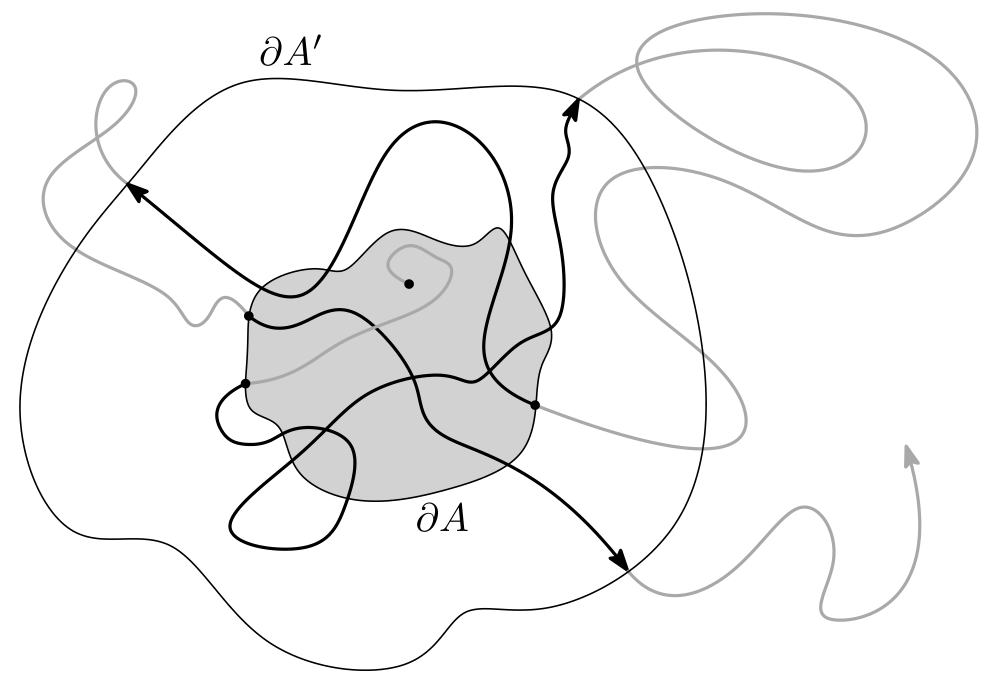
\includegraphics[width=249pt]{../assets/2689/excursions.png}
\caption{Excursions (pictured as bold pieces of trajectories) of random walks between~$\partial A$ and $\partial A'$.}\label{f_excursions}
\end{center}
\end{figure}


\begin{proof}[Proof of Proposition~\ref{p_basic_prop}.]
It is straightforward to check~\eqref{1.1.1}--\eqref{1.1.3} directly, we leave this task for the reader. Item~\eqref{1.1.4} (the transience) follows from~\eqref{1.1.3} and Theorem~2.5.8 of~\cite{MPW17}.

As for~(v), we first observe that~\eqref{escape_from_site} is a consequence of~\eqref{not_hit_site}, although it is of course also possible to prove it directly, see~\cite[Proposition~2.2]{CPV16}. Indeed, using~\eqref{def_hatS} and then~\eqref{not_hit_site}, \eqref{a_harm} and~\eqref{a(x)=1}, one can write
\begin{align*}
\IP_x\big[\htau_1(x)<\infty\big] &= \frac{1}{4a(x)}\sum_{y\sim x} a(y)
\IP_y\big[\htau_1(x)<\infty\big]\\
&= \frac{1}{4a(x)}\sum_{y\sim x} \frac{1}{2}\left(a(y) + a(x) -a(y-x)\right) \\
&= 1 - \frac{1}{2a(x)}.
\end{align*}

Now, to prove~\eqref{not_hit_site}, we essentially use the approach of Lemma~3.7 of~\cite{CPV16}, although here the calculations are simpler. Let us define (note that all the probabilities below are for the simple random walk~$S$)
\begin{align*}
h_1&=\IP_x[\tau_1(0) <\tau_1(R)],\\
h_2&= \IP_x[\tau_1(y) <\tau_1(R)],\\
q_{12}&=\IP_0[\tau_1(y) <\tau_1(R)],\\
q_{21}&=\IP_y[\tau_1(0)<\tau_1(R)],\\
p_1&=\IP_x[\tau_1(0) <\tau_1(R) \wedge \tau_1(y)],\\
p_2&=\IP_x[\tau_1(y) <\tau_1(R) \wedge \tau_1(0)],
\end{align*}
see Figure~\ref{f_pqh12}.

\begin{figure}
\begin{center}
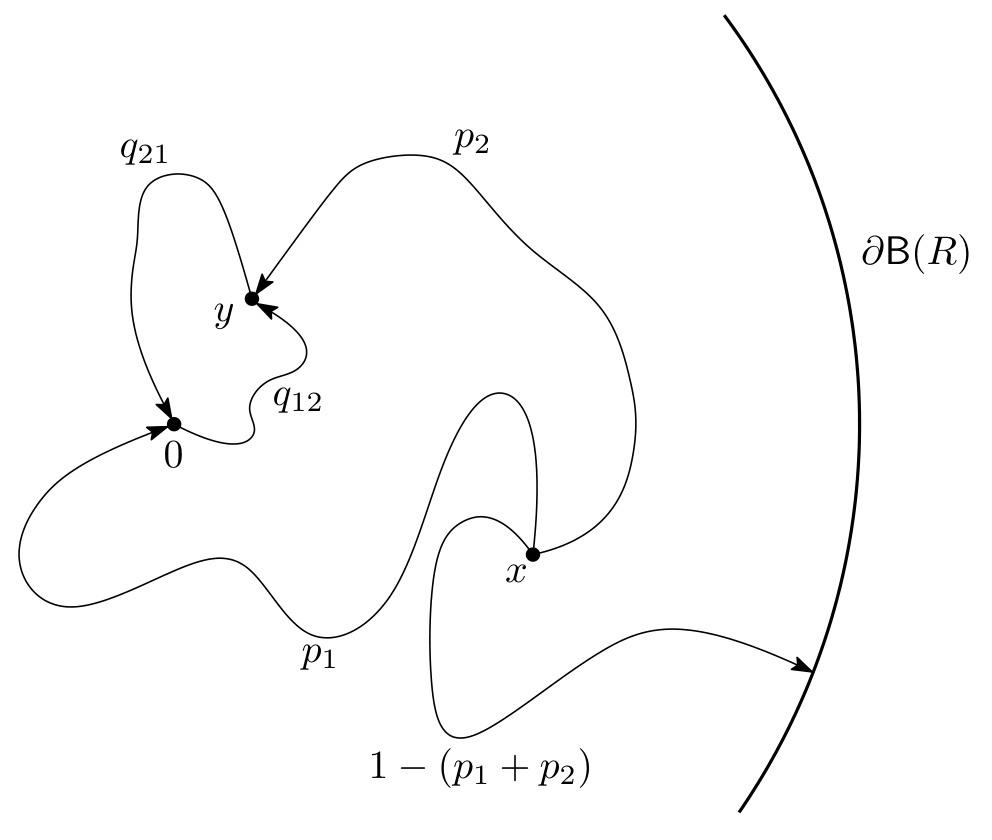
\includegraphics[width=248pt]{../assets/2689/hitting-trajectories.png}
\caption{Trajectories for the probabilities of interest.}\label{f_pqh12}
\end{center}
\end{figure}

Using~\eqref{nothit_r_dim2} (and in addition the Markov property and~\eqref{a_harm} for~\eqref{q12}) we have for $x,y \neq 0$, $x \neq y$
\begin{align}
h_1&=1-\frac{a(x)}{a(R)+O(R^{-1})},\label{h1}
\\
h_2&=1-\frac{a(x-y)}{a(R)+O(R^{-1}\|y\|)},\label{h2}
\\
q_{12}&=1-\frac{a(y)}{a(R)+O(R^{-1}\|y\|)},\label{q12}
\\
q_{21}&=1-\frac{a(y)}{a(R)+O(R^{-1})},\label{q21}
\end{align}
which implies that
\begin{align}
\lim_{R\to\infty} (1-h_1)a(R)&=a(x),\label{lim_h1}
\\
\lim_{R\to\infty} (1-h_2)a(R)&=a(x-y),\label{lim_h2}
\\
\lim_{R\to\infty} (1-q_{12})a(R) &= a(y),\label{lim_q12}
\\
\lim_{R\to\infty} (1-q_{21})a(R) &=a(y).\label{lim_q21}
\end{align}

Observe that, due to the Markov property, it holds that
\begin{align*}
h_1 &= p_1 + p_2q_{21},\\
h_2 &= p_2 + p_1q_{12}.
\end{align*}
Solving these equations with respect to $p_1,p_2$, we obtain
\begin{align}
p_1 &= \frac{h_1-h_2q_{21}}{1-q_{12}q_{21}},\label{expr_p1}
\\
p_2 &= \frac{h_2-h_1q_{12}}{1-q_{12}q_{21}}.\label{expr_p2}
\end{align}
Let us denote
\begin{equation}\label{bar_all}
\hh_1=1-h_1, \quad \hh_2=1-h_2,\quad
\hq_{12}=1-q_{12},\quad \hq_{21}=1-q_{21}.
\end{equation}
Next, using
%~\eqref{h1}--\eqref{q21} together with
Lemma~\ref{l_relation_S_hatS}, we have that
\begin{align}
\IP_x[\htau_1(y)<\htau_1(R)] &= \IP_x[\tau_1(y)<\tau_1(R)\mid \tau_1(R)<\tau_1(0)]
\big(1+o(R^{-1})\big)\nonumber\\
&=\frac{\IP_x[\tau_1(y)<\tau_1(R)<\tau_1(0)]}{\IP_x[\tau_1(R)<\tau_1(0)]}
\big(1+o(R^{-1})\big)\nonumber\\
&=\frac{p_2(1-q_{21})}{1-h_1} \big(1+o(R^{-1})\big)\nonumber\\
&= \frac{(h_2-h_1q_{12})(1-q_{21})}{(1-q_{12}q_{21})(1-h_1)}
\big(1+o(R^{-1})\big)\nonumber\\
&= \frac{(\hh_1+\hq_{12}-\hh_2-\hh_1\hq_{12})\hq_{21}} {(\hq_{12}+\hq_{21}-\hq_{12}\hq_{21})\hh_1} \big(1+o(R^{-1})\big).\label{hat_hq}
\end{align}
Since $\IP_x[\htau_1(y)<\infty]=\lim_{R\to\infty}
\IP_x[\htau_1(y)<\htau_1(R)]$, using~\eqref{lim_h1}--\eqref{lim_q21} we obtain~\eqref{not_hit_site} (observe that the ``product'' terms in~\eqref{hat_hq} are of smaller order and will disappear in the limit).
\end{proof}


We now use the ideas contained in the last proof to obtain some refined bounds on the hitting probabilities for excursions of the conditioned walk.


\begin{figure}
\begin{center}
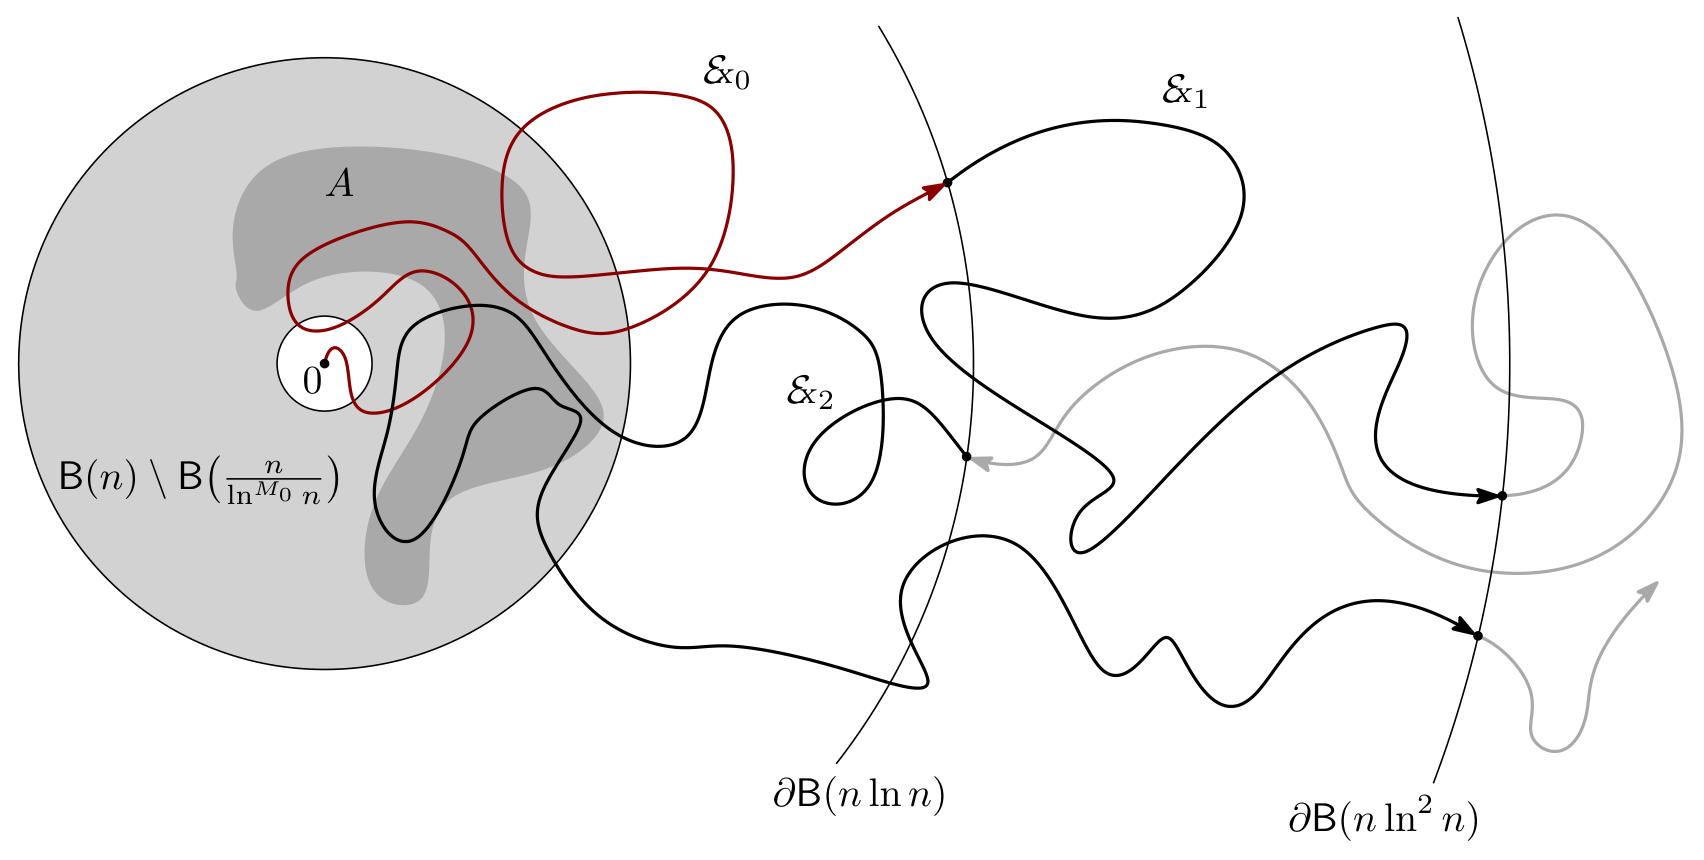
\includegraphics[width=426pt]{../assets/2689/mesoscopic-excursions.png}
\caption{Excursions and their visits to $A$}\label{f_excur_disks}
\end{center}
\end{figure}

Let us assume that $\|x\|\geq n\ln^{-M_0}n$ and $y\in A$, where the set~$A$ is as in Theorem~\ref{t_main_res}. Also, abbreviate $R=n\ln^2 n$.
\begin{lemm}\label{l_refined_probs}
In the above situation, we have
\begin{multline}\label{gen_exc_hit}
\IP_x[\htau_1(y)<\htau_1(R)]
\\ = \big(1+O(\ln^{-3} n)\big)
\frac{a(x)a(R)+a(y)a(R)-a(x-y)a(R)-a(x)a(y)}{a(x)(2a(R)-a(y))}.
\end{multline}
\end{lemm}

\begin{proof}
This is essentially the same calculation as in the proof of~\eqref{not_hit_site}, with the following difference: after arriving to the expression~\eqref{hat_hq}, instead of sending~$R$ to infinity (which conveniently ``kills'' many terms there), we need to carefully deal with all the $O$'s. Specifically, we reuse notations~\eqref{h1}--\eqref{q21} and~\eqref{bar_all}, then write
\begin{align}
\IP_x[\htau_1(y)<\htau_1(R)] &= \IP_x[\tau_1(y)<\tau_1(R)\mid \tau_1(R)<\tau_1(0)]
\big(1+O(n^{-1})\big)\nonumber\\
&= \frac{B_1}{B_2}\big(1+o(n^{-1})\big),\label{B1/B2}
\end{align}
where (observe that, since $\|y\|\leq n$ and $R=n\ln^2 n$, we have $a(R)+O(R^{-1}\|y\|) =a(R)+O(\ln^{-2} n)=a(R)(1+O(\ln^{-3} n)$)
\begin{align*}
B_1 &= (\hh_1+\hq_{12}-\hh_2-\hh_1\hq_{12})\hq_{21}\\
&= \frac{a(y)}{a(R)+O(R^{-1})}
\Big(\frac{a(x)}{a(R)+O(R^{-1})}+\frac{a(y)}{a(R)+O(R^{-1}\|y\|)}\\
& \qquad \qquad \qquad -\frac{a(x-y)}{a(R)+O(R^{-1}\|y\|)} -\frac{a(x)a(y)}{(a(R)+O(R^{-1}))(a(R)+O(R^{-1}\|y\|))}\Big)\\
&= \big(1+O((R\ln R)^{-1})\big)
\frac{a(y)}{a(R)} \cdot
\frac{a(x)a(R)+a(y)a(R)-a(x-y)a(R)-a(x)a(y)}{(1+O(\ln^{-3} n))a^2(R)}\\
&= \big(1+O(\ln^{-3} n)\big)
\frac{a(y)}{a(R)} \cdot
\frac{a(x)a(R)+a(y)a(R)-a(x-y)a(R)-a(x)a(y)}{a^2(R)},
\end{align*}
and
\begin{align*}
B_2 &= (\hq_{12}+\hq_{21}-\hq_{12}\hq_{21})\hh_1\\
&= \frac{a(x)}{a(R)+O(R^{-1})}
\Big(\frac{a(y)}{a(R)+O(R^{-1}\|y\|)}+\frac{a(y)}{a(R)+O(R^{-1})}\\
& \qquad \qquad \qquad \qquad \qquad -\frac{a^2(y)}{(a(R)+O(R^{-1}))(a(R)+O(R^{-1}\|y\|))}\Big)\\
&=\big(1+O((R\ln R)^{-1})\big)
\frac{a(x)}{a(R)} \cdot
\frac{2a(y)a(R)-a^2(y)+O(\ln^{-1}n)}{(1+O(\ln^{-3} n))a^2(R)}\\
&= \big(1+O(\ln^{-3} n)\big)
\frac{a(x)}{a(R)} \cdot \frac{2a(y)a(R)-a^2(y)}{a^2(R)}.
\end{align*}
We insert the above back to~\eqref{B1/B2} and note that the factor $\frac{a(y)}{a^3(R)}$ cancels to obtain~\eqref{gen_exc_hit}.
\end{proof}


\section{Proofs of the main results}\label{s_proofs}

We start with

\begin{proof}[Proof of Theorem~\ref{t_main_res}]
First, we describe informally the idea of the proof. We consider the visits to the set $A$ during excursions of the walk from $\partial\B(n\ln n)$ to $\partial\B(n\ln^2 n)$, see Figure~\ref{f_excur_disks}. The crucial argument is the following: the randomness of~$\V(A)$ comes from the \emph{number} of excursions and not from the excursions themselves. If the number of excursions is around $c\times\frac{\ln n}{\ln\ln n}$, then it is possible to show (using a standard weak-LLN argument) that the proportion of uncovered sites in~$A$ is \emph{concentrated} around~$e^{-c}$. On the other hand, that number of excursions can be modeled roughly as $Y \times\frac{\ln n}{\ln\ln n}$, where~$Y$ is an Exponential($1$) random variable. Then, $\IP[\V(A)\leq s]\approx \IP[Y\geq \ln s^{-1}]=s$, as required.

We now give a rigorous argument. Let $\hH$ be the conditional entrance measure for the (conditioned) walk~$\s$, i.e.,
\begin{equation}\label{df_hatH}
\hH_A(x,y) = \IP_x\big[\s_{\htau_1(A)}=y \mid \htau_1(A)<\infty\big].
\end{equation}
Let us first denote the initial piece of the trajectory by $\Ex_0=\s_{[0,\htau(n\ln n)]}$. Then, we consider a \emph{Markov chain} $(\Ex_k,k\geq 1)$ of excursions between $\partial\B(n\ln n)$ and $\partial\B(n\ln^2 n)$, defined in the following way: for $k\geq 2$ the initial site of~$\Ex_k$ is chosen according to the measure~$\hH_{\B(n\ln n)}(z_{k-1},\cdot\,)$, where $z_{k-1}\in\partial\B(n\ln^2 n)$ is the last site of the excursion~$\Ex_{k-1}$; also, the initial site of~$\Ex_1$ is the last site of $\Ex_0$; the weights of trajectories are chosen according to~\eqref{def_hatS} (i.e., each excursion is an $\s$-walk trajectory). It is important to observe that one may couple $(\Ex_k,k\geq 1)$ with the ``true'' excursions of the walk~$\s$ in an obvious way: one just picks the excursions subsequently, each time tossing a coin to decide if the walk returns to $\B(n\ln n)$.

Let
\[
\psi_n = \min_{x\in\partial\B(n\ln^2 n)}\IP_x[\htau(n\ln n)=\infty]
\]
be the \emph{minimal} probability to avoid $\B(n\ln n)$, starting at sites of $\partial\B(n\ln^2 n)$. Using~\eqref{escape_condS} it is straightforward to obtain that
\[
\IP_x[\htau_1(n\ln n)=\infty] = \frac{\ln\ln n}{\ln n + 2\ln\ln n}\big(1+O(n^{-1})\big)
\]
for any $x\in \partial\B(n\ln^2 n)$, and so it also holds that
\begin{equation}\label{oc_psi_n}
\psi_n = \frac{\ln\ln n}{\ln n + 2\ln\ln n}\big(1+O(n^{-1})\big).
\end{equation}
Let us consider a sequence of i.i.d.\ random variables $(\eta_k,k\geq 0)$ such that $\IP[\eta_k=1]=1-\IP[\eta_k=0]=\psi_n$. Let $\hN = \min\{k:\eta_k = 1\}$, so that~$\hN$ is a Geometric random variable with mean~$\psi_n^{-1}$. Now, \eqref{oc_psi_n} implies that $\IP_x[\htau(n\ln n)=\infty]-\psi_n\leq O\big(\frac{\ln\ln n}{n\ln n}\big)$ for any $x\in \partial\B(n\ln^2 n)$, so it is clear\footnote{Let $(Z_n,n\geq 1)$ be a sequence of $\{0,1\}$-valued random variables adapted to a filtration $(\FFF_n,n\geq 1)$ and such that $\IP[Z_{n+1}=1\mid \FFF_n]\in [p,p+\eps]$ a.s.. Then it is elementary to obtain that the total variation distance between the random variable $\min\{k: Z_k=1\}$ and the Geometric random variable with mean~$p^{-1}$ is bounded above by $O(\eps/ p)$.} that~$\hN $ can be coupled with the actual number of excursions~$N$ in such a way that $N\leq \hN $ a.s.\ and
\begin{equation}\label{N_neq_hatN}
\IP[N \neq \hN] \leq O(n^{-1}).
\end{equation}
Note that this construction preserves the independence of~$\hN$ from the excursion sequence $(\Ex_k,k\geq 1)$ itself.

Define
\begin{align*}
\RR^{(k)} &= \frac{\big|A\cap (\Ex_0\cup \Ex_1\cup \ldots \cup \Ex_k)\big|}{|A|},
\intertext{and}
\V^{(k)} &= \frac{\big|A\setminus (\Ex_0\cup \Ex_1\cup \ldots \cup \Ex_k)\big|}{|A|}=1-\RR^{(k)}
\end{align*}
to be the proportions of visited and unvisited sites in~$A$ with respect to the first~$k$ excursions together with the initial piece~$\Ex_0$.

Now, it is straightforward to check that~\eqref{gen_exc_hit} implies that, for any $x\in \partial\B(n\ln n)$ and $y \in A$
\begin{equation}\label{hit_y}
\IP_x\big[\htau_1(y)<\htau_1(n\ln^2 n)\big] = \frac{\ln\ln n}{\ln n}
\Big(1+O\Big(\frac{\ln\ln n}{\ln n}\Big)\Big),
\end{equation}
and, for $y,z\in \B(n)\setminus\B\big(\frac{n}{2\ln^{M_0}n}\big)$ such that $\|y-z\| = n/b$ with $b\leq 2\ln^{M_0}n$
\begin{equation}\label{hit_z}
\IP_z\big[\htau_1(y)<\htau_1(n\ln^2 n)\big] =
\frac{2\ln\ln n + \ln b}{\ln n}
\Big(1+O\Big(\frac{\ln\ln n}{\ln n}\Big)\Big).
\end{equation}
Indeed, first, observe that the factor~$B_2$ in~\eqref{gen_exc_hit} is, in both cases,
\begin{equation}\label{ocenka_B2}
a(x)(2a(R)-a(y)) = \Big(\frac{2}{\pi}\Big)^2
\ln^2 n + O\big(\ln n\ln\ln n\big).
\end{equation}
As for the factor~$B_1$, we have
\begin{align*}
B_1 &= a(x)a(R)+a(y)a(R)-a(x-y)a(R)-a(x)a(y)\\
&= (a(x)-a(x-y))a(R) - (a(R)-a(x))a(y)\\
&= O\big((\ln n)^{-1}\big)\times O(\ln n) + \Big(\frac{2}{\pi}\ln\ln n + o(n^{-2})\Big)
\times \Big(\frac{2}{\pi}\ln n + O(\ln\ln n)\Big)\\
&= \Big(\frac{2}{\pi}\Big)^2
\ln n\ln\ln n + O\big((\ln\ln n)^2\big)
\end{align*}
in the case of~\eqref{hit_y}, and (writing also $\|z\|=n/c$ with $(2\ln^{M_0} n)^{-1}\leq c\leq 1$)
\begin{align*}
B_1 &= a(z)a(R)+a(y)a(R)-a(z-y)a(R)-a(z)a(y)\\
&= (a(z)-a(z-y))a(R) - (a(R)-a(z))a(y)\\
&= \frac{2}{\pi}\big(-\ln c +\ln b + o(n^{-1})\big)
\times \frac{2}{\pi}\big(\ln n + O(\ln\ln n)\big)\\
& \qquad + \frac{2}{\pi}\big(2\ln\ln n +\ln c + o(n^{-1})\big)
\times \Big(\frac{2}{\pi}\ln n + O(\ln\ln n)\Big)\\
&= \Big(\frac{2}{\pi}\Big)^2
\ln n\times(2\ln\ln n + \ln b) + O\big((\ln\ln n)^2\big)
\end{align*}
in the case of~\eqref{hit_z}; with~\eqref{ocenka_B2} we then obtain~\eqref{hit_y}--\eqref{hit_z}.

For $y\in A$ and a fixed~$k\geq 1$ consider the random variable
\[
\xi_y^{(k)} = \1{y\notin\Ex_0\cup \Ex_1\cup \ldots \cup \Ex_k},
\]
so that $\V^{(k)} = |A|^{-1}\sum_{y\in A}\xi_y^{(k)}$. Now~\eqref{hit_y} implies that, for all $j\geq 1$,
\[
\IP[y\notin \Ex_j] = 1-\frac{\ln\ln n}{\ln n}
\Big(1+O\Big(\frac{\ln\ln n}{\ln n}\Big)\Big),
\]
and~\eqref{hit_z} implies that
\[
\IP[y\notin \Ex_0\cup\Ex_1] = 1 - O\Big(\frac{\ln\ln n}{\ln n}\Big)
\]
for any~$y\in A$. Let $\mu_y^{(k)}=\IE \xi_y^{(k)}$. Then we have
\begin{align}
\mu_y^{(k)} &= \IP[y\notin\Ex_0\cup \Ex_1\cup \ldots \cup \Ex_k]
\nonumber\\
&= \Big(1-O\Big(\frac{\ln\ln n}{\ln n}\Big)\Big)
\times
\Bigg(\Big(1-\frac{\ln\ln n}{\ln n}
\Big(1+O\Big(\frac{\ln\ln n}{\ln n}\Big)\Big)\Big)
\Bigg)^{k-1}\nonumber\\
&= \exp\Big(-k\frac{\ln\ln n}{\ln n}
\Big(1+O\Big(k^{-1}+\frac{\ln\ln n}{\ln n}\Big)\Big)\Big).\label{est_mu_k}
\end{align}
Next, we need to estimate the covariance of~$\xi_y^{(k)}$ and~$\xi_z^{(k)}$ in case $\|y-z\|\geq n\ln^{-M_0}n$. First note that, for any $x\in \partial\B(n\ln n)$
\begin{align*}
\IP_x\big[\{y,z\}\cap \Ex_1 = \emptyset \big] &= 1-\IP_x[y\in\Ex_1] - \IP_x[z\in\Ex_1] + \IP_x\big[\{y,z\}\subset \Ex_1 \big]\\
&= 1- 2 \frac{\ln\ln n}{\ln n}
\Big(1+O\Big(\frac{\ln\ln n}{\ln n}\Big)\Big) + \IP_x\big[\{y,z\}\subset \Ex_1 \big]
\end{align*}
by~\eqref{hit_y}; also, since
\begin{multline*}
\big\{\htau_1(y)<\htau_1(z)<\htau_1(n\ln^2 n)\big\} \\
\subset
\big\{\htau_1(y)<\htau_1(n\ln^2 n),\s_k=z \text{ for some }
\htau_1(y)<k<\htau_1(n\ln^2 n)\big\}
\end{multline*}
from~\eqref{hit_y}--\eqref{hit_z} we obtain
\begin{align*}
\IP_x\big[\{y,z\}\subset \Ex_1 \big] &=
\IP_x\big[\max\{\htau_1(y),\htau_1(z)\}<\htau_1(n\ln^2 n)\big]
\\
&= \IP_x\big[\htau_1(y)<\htau_1(z)<\htau_1(n\ln^2 n)\big] + \IP_x\big[\htau_1(z)<\htau_1(y)<\htau_1(n\ln^2 n)\big]\\
&\leq \IP_x\big[\htau_1(y)<\htau_1(n\ln^2 n)\big]
\IP_y\big[\htau_1(z)<\htau_1(n\ln^2 n)\big]\\
& \qquad + \IP_x\big[\htau_1(z)<\htau_1(n\ln^2 n)\big]
\IP_z\big[\htau_1(y)<\htau_1(n\ln^2 n)\big]\\
&\leq 2\frac{\ln\ln n}{\ln n} \times \frac{(2+M_0)\ln\ln n}{\ln n}
\Big(1+O\Big(\frac{\ln\ln n}{\ln n}\Big)\Big)\\
&= O\Big(\Big(\frac{\ln\ln n}{\ln n}\Big)^2\Big).
\end{align*}
Therefore, similarly to~\eqref{est_mu_k} we obtain
\begin{align*}
\IE(\xi_y^{(k)}\xi_z^{(k)}) &= \exp\Big(-2k\frac{\ln\ln n}{\ln n}
\Big(1+O\Big(k^{-1}+\frac{\ln\ln n}{\ln n}\Big)\Big)\Big),
\end{align*}
which, together with~\eqref{est_mu_k}, implies after some elementary calculations that, for all~$y,z\in A$ such that $\|y-z\|\geq n\ln^{-M_0}n$
\begin{equation}\label{est_cov}
\cov (\xi_y^{(k)},\xi_z^{(k)}) = O\Big(\frac{\ln\ln n}{\ln n}\Big)
\end{equation}
uniformly in~$k$, since
\[
\Bigg(\frac{\ln\ln n}{\ln n} + k\Big(\frac{\ln\ln n}{\ln n}\Big)^2
\Bigg) \exp\Big(-2k\frac{\ln\ln n}{\ln n}\Big) = O\Big(\frac{\ln\ln n}{\ln n}\Big)
\]
uniformly in~$k$. Recall the notation~$\ell^{(n)}_A$ from~\eqref{df_ell_A}. Now, using Chebyshev's inequality, we write
\begin{align}
\IP\Big[\Big|&|A|^{-1}\sum_{y\in A}(\xi_y^{(k)} -\mu_y^{(k)})\Big|>\eps\Big]\nonumber\\
&\leq (\eps|A|)^{-2} \Var \left(\sum_{y\in A}\xi_y^{(k)}\right)
\nonumber\\
&= (\eps|A|)^{-2} \sum_{y,z\in A}\cov (\xi_y^{(k)},\xi_z^{(k)})
\nonumber\\
&= (\eps|A|)^{-2} \Bigg(\sum_{\substack{y,z\in A,\\
\|y-z\|< \frac{n}{\ln^{M_0}n}}} \cov (\xi_y^{(k)},\xi_z^{(k)}) + \sum_{\substack{y,z\in A,\\
\|y-z\|\geq \frac{n}{\ln^{M_0}n}}}
\cov (\xi_y^{(k)},\xi_z^{(k)}) \Bigg)
\nonumber\\
&\leq (\eps|A|)^{-2} \left(\sum_{y\in A} \big|A\cap \B(y,\tfrac{n}{\ln^{M_0}n})\big| + |A|^2 O\Big(\frac{\ln\ln n}{\ln n}\Big) \right)\nonumber\\
&\leq \eps^{-2}
\ell^{(n)}_A + \eps^{-2} O\Big(\frac{\ln\ln n}{\ln n} \Big).\label{bigcalc_Cheb}
\end{align}

Let
\[
\Phi^{(s)} = \min\big\{k: \V^{(k)}\leq s\big\}
\]
be the number of excursions necessary to make the unvisited proportion of~$A$ at most~$s$. We have
\begin{align*}
\IP[\V(A)\leq s] & = \IP[\Phi^{(s)}\leq N]\\
&= \IP[\Phi^{(s)}\leq N,N=\hN] +
\IP[\Phi^{(s)}\leq N,N\neq \hN]\\
&= \IP[\Phi^{(s)}\leq \hN] + \IP[\Phi^{(s)}\leq N,N\neq \hN] - \IP[\Phi^{(s)}\leq \hN,N\neq \hN],
\end{align*}
so, recalling~\eqref{N_neq_hatN},
\begin{equation}\label{V_Phi_hatN}
\big|\IP[\V(A)\leq s] - \IP[\Phi^{(s)}\leq \hN]\big|
\leq \IP[N\neq \hN] \leq O(n^{-1}).
\end{equation}

Next, we write
\begin{align}
\IP[\Phi^{(s)}\leq \hN] &= \IE \big(\IP[\hN \geq \Phi^{(s)}\mid\Phi^{(s)}]\big)\nonumber \\
&=\IE (1-\psi_n)^{\Phi^{(s)}},\label{genfunc}
\end{align}
(here we used the independence property stated below~\eqref{N_neq_hatN}) and concentrate on obtaining lower and upper bounds on the expectation in the right-hand side of~\eqref{genfunc}. For this, assume that $s\in(0,1)$ is fixed and abbreviate
\begin{align*}
\delta_n &= \Big(\frac{\ln\ln n}{\ln n}\Big)^{1/3}\\
k_n^{-} &= \Big\lfloor(1-\delta_n)\ln s^{-1} \frac{\ln n}{\ln\ln n}
\Big\rfloor,\\
k_n^{+} &= \Big\lceil(1+\delta_n)\ln s^{-1} \frac{\ln n}{\ln\ln n}
\Big\rceil;
\end{align*}
we also assume that~$n$ is sufficiently large so that $\delta_n \in(0,\frac{1}{2})$ and $1<k_n^{-}<k_n^{+}$. Now, according to~\eqref{est_mu_k},
\begin{align*}
\mu_y^{(k_n^{\pm})} &= \exp\Big(-(1\pm \delta_n)\ln s^{-1}
\Big(1+O\Big((k_n^{\pm})^{-1}+\frac{\ln\ln n}{\ln n}\Big)\Big)\Big)\\
& = s \exp\Big(-\ln s^{-1}
\Big(\pm \delta_n+O\Big((k_n^{\pm})^{-1}+\frac{\ln\ln n}{\ln n}\Big)\Big)\Big)\\
& = s \Big(1+O\Big(\delta_n\ln s^{-1} + \frac{\ln\ln n}{\ln n}(1+\ln s^{-1})\Big)\Big),
\end{align*}
so in both cases it holds that (observe that $s\ln s^{-1}\leq 1/e$ for all $s\in[0,1]$)
\begin{equation}\label{muk_ourcase}
\mu_y^{(k_n^{\pm})} = s + O\Big(\delta_n +\frac{\ln\ln n}{\ln n} \Big) = s + O(\delta_n).
\end{equation}
With a similar calculation, one can also observe that
\begin{equation}\label{1-psi_ourcase}
(1-\psi_n)^{(k_n^{\pm})} = s + O(\delta_n).
\end{equation}

We then write, using~\eqref{muk_ourcase}
\begin{align}
\IP[\Phi^{(s)} > k_n^{+}] &= \IP[\V^{(k_n^{+})}>s]\nonumber\\
&= \IP\Big[|A|^{-1}\sum_{y\in A}\xi_y^{(k_n^{+})}> s\Big]\nonumber\\
&= \IP\Big[|A|^{-1}\sum_{y\in A}(\xi_y^{(k_n^{+})} -\mu_y^{(k_n^{+})})> s - |A|^{-1}\sum_{y\in A}\mu_y^{(k_n^{+})}\Big]\nonumber\\
&= \IP\Big[|A|^{-1}\sum_{y\in A}(\xi_y^{(k_n^{+})} -\mu_y^{(k_n^{+})})> O(\delta_n)
\Big].\label{Cheb+}
\end{align}
Then, \eqref{bigcalc_Cheb} implies that
\begin{equation}\label{est_k+}
\IP[\Phi^{(s)} > k_n^{+}]
\leq O\Big(\ell^{(n)}_A\Big(\frac{\ln\ln n}{\ln n}\Big)^{-2/3} + \Big(\frac{\ln\ln n}{\ln n}\Big)^{1/3} \Big).
\end{equation}
Quite analogously, one can also obtain that
\begin{equation}\label{est_k-}
\IP[\Phi^{(s)} < k_n^{-}]
\leq O\Big(\ell^{(n)}_A\Big(\frac{\ln\ln n}{\ln n}\Big)^{-2/3} + \Big(\frac{\ln\ln n}{\ln n}\Big)^{1/3} \Big).
\end{equation}
Using~\eqref{1-psi_ourcase} and~\eqref{est_k+}, we then write
\begin{align}
\IE (1-\psi_n)^{\Phi^{(s)}} &\geq
\IE \big((1-\psi_n)^{\Phi^{(s)}}\1{\Phi^{(s)} \leq k_n^{+}}\big)
\nonumber\\
&\geq (1-\psi_n)^{k_n^{+}}
\IP[\Phi^{(s)} \leq k_n^{+}]\nonumber\\
&\geq \Big(s-O\Big(\Big(\frac{\ln\ln n}{\ln n}\Big)^{1/3}\Big)\Big)
\Big(1-O\Big(\ell^{(n)}_A\Big(\frac{\ln\ln n}{\ln n}\Big)^{-2/3} + \Big(\frac{\ln\ln n}{\ln n}\Big)^{1/3} \Big)\Big),\label{bigest>}
\end{align}
and, using~\eqref{1-psi_ourcase} and~\eqref{est_k-},
\begin{align}
\IE (1-\psi_n)^{\Phi^{(s)}} &=
\IE \big((1-\psi_n)^{\Phi^{(s)}}\1{\Phi^{(s)} \geq k_n^{-}}\big) + \IE \big((1-\psi_n)^{\Phi^{(s)}}\1{\Phi^{(s)} < k_n^{-}}\big)
\nonumber\\
&\leq (1-\psi_n)^{k_n^{-}} + \IP[\Phi^{(s)} < k_n^{-}]
\nonumber\\
&\leq \Big(s+O\Big(\Big(\frac{\ln\ln n}{\ln n}\Big)^{1/3}\Big)\Big)
\nonumber\\
& \qquad +
\Big(1-O\Big(\ell^{(n)}_A\Big(\frac{\ln\ln n}{\ln n}\Big)^{-2/3} + \Big(\frac{\ln\ln n}{\ln n}\Big)^{1/3} \Big)\Big).\label{bigest<}
\end{align}


Therefore, using also~\eqref{V_Phi_hatN}--\eqref{genfunc}, we obtain~\eqref{main_res}, thus concluding the proof of Theorem~\ref{t_main_res}.
\end{proof}

Next, we will prove Theorems~\ref{t_rec_trans} and~\ref{t_Liouville}, since the latter will be needed in the course of the proof of Theorem~\ref{t_bigholes}.

\begin{proof}[Proof of Theorem~\ref{t_rec_trans}]
Clearly, we only need to prove that every infinite subset of~$\Z^d$ is recurrent for~$\s$. Basically, this is a consequence of the fact that, due to~\eqref{not_hit_site},
\begin{equation}\label{lim1/2}
\lim_{y\to\infty} \IP_{x_0}\big[\htau_1(y)<\infty\big] = \frac{1}{2}
\end{equation}
for any $x_0\in\Z^2$. Indeed, let~$\s_0=x_0$; since~$A$ is infinite, by~\eqref{lim1/2} one can find~$y_0\in A$ and~$R_0$ such that $\{x_0,y_0\}\subset \B(R_0)$ and
\[
\IP_{x_0}\big[\htau_1(y_0)<\htau_1(R_0)\big] \geq \frac{1}{3}.
\]
Then, for any~$x_1\in \partial\B(R_0)$, we can find~$y_1\in A$ and~$R_1>R_0$ such that $y_1\in \B(R_1)\setminus \B(R_0)$ and
\[
\IP_{x_1}\big[\htau_1(y_1)<\htau_1(R_1)\big] \geq \frac{1}{3}.
\]
Continuing in this way, we can construct a sequence $R_0<R_1<R_2<\ldots$ (depending on the set~$A$) such that, for each $k\geq 0$, the walk~$\s$ hits~$A$ on its way from~$\partial\B(R_k)$ to~$\partial\B(R_{k+1})$ with probability at least~$\frac{1}{3}$, regardless of the past. This clearly implies that~$A$ is a recurrent set.
\end{proof}

\begin{proof}[Proof of Theorem~\ref{t_Liouville}]
Indeed, Theorem~\ref{t_rec_trans} implies that every subset of~$\Z^2$ must be either recurrent or transient, and then Proposition~3.8 in~\cite[Chapter~2]{R84} implies the Liouville property. Still, for the reader's convenience, we include the proof here. Assume that $h:\Z^2\setminus\{0\} \to \R$ is a bounded harmonic function for~$\s$. Let us prove that
\begin{equation}\label{limit_infty}
\liminf_{y\to \infty}h(y) = \limsup_{y\to \infty}h(y),
\end{equation}
that is, $h$ must have a limit at infinity. Indeed, assume that~\eqref{limit_infty} does not hold, which means that there exist two constants~$b_1<b_2$ and two \emph{infinite} sets $B_1,B_2\subset\Z^2$ such that $h(y)\leq b_1$ for all $y\in B_1$ and $h(y) \geq b_2$ for all $y\in B_2$. Now, on one hand~$h(\s_n)$ is a bounded martingale, so it must a.s.\ converge to some limit; on the other hand, Theorem~\ref{t_rec_trans} implies that both~$B_1$ and~$B_2$ will be visited infinitely often by~$\s$, and so~$h(\s_n)$ cannot converge to any limit, thus yielding a contradiction. This proves~\eqref{limit_infty}.

Now, if $\lim_{y\to \infty}h(y)=c$, then it is easy to obtain from the Maximum Principle that $h(x)=c$ for any~$x$. This concludes the proof of Theorem~\ref{t_Liouville}.
\end{proof}

Finally, we are able to prove that there are ``big holes'' in the range of~$\s$:
\begin{proof}[Proof of Theorem~\ref{t_bigholes}]
Clearly, if~$G$ does not surround the origin in the sense of Definition~\ref{df_surround}, then $G\subset \B(c_1)\setminus \B(c_3)$. For the sake of simplicity, let us assume that $G\subset\B(1)\setminus \B(1/2)$; the general case can be treated in a completely analogous way.

Consider the two sequences of events
\begin{align*}
E_n &= \big\{\htau_1(2^{3n-1}G)>\htau_1(2^{3n}),
\|\s_j\| > 2^{3n-1} \text{ for all } j\geq \htau_1(2^{3n})\big\},\\
E'_n &= \big\{
\|\s_j\| > 2^{3n-1} \text{ for all } j\geq \htau_1(2^{3n})\big\}
\end{align*}
and note that $E_n\subset E'_n$ and $2^{3n-1}G\cap \s_{[0,\infty)}=\emptyset$ on~$E_n$. Our goal is to show that a.s.\ an infinite number of events $(E_n, n\geq 1)$ occurs. Observe, however, that the events in each of the above two sequences are \emph{not} independent, so the ``basic'' second Borel--Cantelli lemma will not work.

In the following, we use a generalization of the second Borel--Cantelli lemma, known as the Kochen--Stone theorem~\cite{KS64}: it holds that
\begin{equation}\label{Kochen--Stone}
\IP\Big[\sum_{k=1}^\infty \1{E_k}=\infty\Big] \geq
\limsup_{k\to\infty} \frac{\big(\sum_{i=1}^k\IP[E_i]\big)^2} {\sum_{i,j=1}^k\IP[E_i\cap E_j]}.
\end{equation}

We will now prove that there exists a positive constant~$c_4$ such that
\begin{equation}\label{lower_En}
\IP[E_n] \geq \frac{c_4}{n} \quad \text{ for all }n\geq 1.
\end{equation}
Indeed, since $G\subset\B(1)\setminus \B(1/2)$ does not surround the origin, by comparison with Brownian motion it is elementary to obtain that, for some~$c_5>0$,
\[
\IP_x\big[\tau_1(2^{3n-1}G)>\tau_1(2^{3n}),
\tau_1(0)>\tau_1(2^{3n}) \big] > c_5
\]
for all~$x\in\partial \B(2^{3(n-1)})$. Lemma~\ref{l_relation_S_hatS} then implies that, for some~$c_6>0$,
\begin{align}
\IP_x\big[&\htau_1(2^{3n-1}G)>\htau_1(2^{3n})\big]\nonumber\\
&= \big(1+o(2^{-3n})\big)
\IP_x\big[\tau_1(2^{3n-1}G)>\tau_1(2^{3n})
\mid \tau_1(0)>\tau_1(2^{3n})\big] \nonumber\\
&= \big(1+o(2^{-3n})\big)
\IP_x\big[\tau_1(2^{3n-1}G)>\tau_1(2^{3n}),
\tau_1(0)>\tau_1(2^{3n})\big] > c_6\label{inv_pri>c}
\end{align}
for all~$x\in\partial \B(2^{3(n-1)})$. Let us denote, recalling~\eqref{formula_for_a}, $\gamma^{*}=\frac{\pi}{2}\times\frac{1}{\ln 2} \times
\frac{2\gamma+ 3\ln 2}{\pi} =\frac{2\gamma+ 3\ln 2}{2\ln 2}$. Using~\eqref{escape_condS}, we then obtain
\begin{align}
\IP_z\big[\|\s_j\| > 2^{3n-1} \text{ for all } j\geq 0\big] & = 1- \frac{a(2^{3n-1})+O(2^{-3n})}{a(2^{3n})+O(2^{-3n})}
\nonumber\\
&= \frac{1}{3n+\gamma^{*}}\big(1+o(2^{-3n})\big).\label{>c/n}
\end{align}
for any $z\in\partial \B(2^{3n})$. The inequality~\eqref{lower_En} follows from~\eqref{inv_pri>c} and~\eqref{>c/n}.

Now, we need an upper bound for $\IP[E_m\cap E_n]$, $m\leq n$. Clearly, $E_m \cap E_n\subset E'_m \cap E'_n$, and note that the event~$E'_m \cap E'_n$ means that the particle hits $\partial\B(2^{3n})$ before $\partial\B(2^{3m-1})$ starting from a site on~$\partial\B(2^{3m})$, and then never hits $\partial\B(2^{3n-1})$ starting from a site on~$\partial\B(2^{3n})$. So, again using~\eqref{escape_condS} and Lemma~\ref{l_relation_S_hatS}, we write analogously to~\eqref{>c/n} (and also omitting a couple of lines of elementary calculations)
\begin{align}
\IP[E_m \cap E_n] & \leq \IP[E'_m \cap E'_n]\nonumber\\
& = \frac{(a(2^{3m-1}))^{-1}-(a(2^{3m}))^{-1}+O(2^{-3m})} {(a(2^{3m-1}))^{-1}-(a(2^{3n}))^{-1}+O(2^{-3m})}
\times \Big(1- \frac{a(2^{3n-1})+O(2^{-3n})}{a(2^{3n})+O(2^{-3n})}\Big)
\nonumber\\
& = \frac{1}{(3(n-m)+1)(3m+\gamma^{*})}\big(1+o(2^{-3m})\big).\label{EmEn_upper}
\end{align}

Now, \eqref{lower_En} implies that $\sum_{i=1}^k\IP[E_i]\geq c_{9}\ln k$, and~\eqref{EmEn_upper} implies (again, after some elementary calculations) that $\sum_{i,j=1}^k\IP[E_i\cap E_j]\leq c_{10}\ln^2 k$. So, using~\eqref{Kochen--Stone}, we obtain that
\[
\IP\Big[\sum_{k=1}^\infty \1{E_k}=\infty\Big] \geq c_{11}>0.
\]
Now, note that, again due to Proposition~3.8 in~\cite[Chapter~2]{R84}, the Liouville property implies that every tail event must have probability~$0$ or~$1$, and so the probability in the above display must be equal to~$1$. This concludes the proof of Theorem~\ref{t_bigholes}.
\end{proof}

\begin{thebibliography}{MMMMMM}
\bibitem[CP17]{CP16} Comets, Francis; Popov, Serguei The vacant set of two-dimensional critical random interlacement is infinite, Ann. Probab., Volume 45 (2017) no. 6B, pp. 4752-4785 \href{https://ahl.centre-mersenne.org/item/AHL_2019__2__349_0/#CP16}{Publisher reference}.
\bibitem[CPV16]{CPV16} Comets, Francis; Popov, Serguei; Vachkovskaia, Marina Two-dimensional random interlacements and late points for random walks, Commun. Math. Phys., Volume 343 (2016) no. 1, pp. 129-164 \href{https://ahl.centre-mersenne.org/item/AHL_2019__2__349_0/#CPV16}{Publisher reference}.
\bibitem[DRS14]{DRS14} Drewitz, Alexander; Ráth, Balázs; Sapozhnikov, Artëm An introduction to random interlacements, SpringerBriefs in Mathematics, Springer, 2014 \href{https://ahl.centre-mersenne.org/item/AHL_2019__2__349_0/#DRS14}{Publisher reference}.
\bibitem[KS64]{KS64} Kochen, Simon; Stone, Charles A note on the Borel-Cantelli lemma, Ill. J. Math., Volume 8 (1964), pp. 248-251 \href{https://ahl.centre-mersenne.org/item/AHL_2019__2__349_0/#KS64}{Publisher reference}.
\bibitem[LL10]{LL10} Lawler, Gregory F.; Limic, Vlada Random walk: a modern introduction, Cambridge Studies in Advanced Mathematics, 123, Cambridge University Press, 2010 \href{https://ahl.centre-mersenne.org/item/AHL_2019__2__349_0/#LL10}{Publisher reference}.
\bibitem[MPW17]{MPW17} Menshikov, Mikhail; Popov, Serguei; Wade, Andrew Non-homogeneous random walks: Lyapunov function methods for near-critical stochastic systems, Cambridge Tracts in Mathematics, 209, Cambridge University Press, 2017 \href{https://ahl.centre-mersenne.org/item/AHL_2019__2__349_0/#MPW17}{Publisher reference}.
\bibitem[PT15]{SLT} Popov, Serguei; Teixeira, Augusto Soft local times and decoupling of random interlacements, J. Eur. Math. Soc., Volume 17 (2015) no. 10, pp. 2545-2593 \href{https://ahl.centre-mersenne.org/item/AHL_2019__2__349_0/#SLT}{Publisher reference}.
\bibitem[Rev84]{R84} Revuz, Daniel Markov chains, North-Holland Mathematical Library, 11, North-Holland, 1984 \href{https://ahl.centre-mersenne.org/item/AHL_2019__2__349_0/#R84}{Publisher reference}.
\bibitem[Szn10]{Szn10} Sznitman, Alain-Sol Vacant set of random interlacements and percolation, Ann. Math., Volume 171 (2010) no. 3, pp. 2039-2087 \href{https://ahl.centre-mersenne.org/item/AHL_2019__2__349_0/#Szn10}{Publisher reference}.
\bibitem[Woe09]{Woess09} Woess, Wolfgang Denumerable Markov chains. Generating functions, boundary theory, random walks on trees, EMS Textbooks in Mathematics, European Mathematical Society, 2009 \href{https://ahl.centre-mersenne.org/item/AHL_2019__2__349_0/#Woess09}{Publisher reference}.
\bibitem[ČT12]{CT12} Černý, Jiří; Teixeira, Augusto Q. From random walk trajectories to random interlacements, Ensaios Matemáticos, 23, Sociedade Brasileira de Matemática, 2012 \href{https://ahl.centre-mersenne.org/item/AHL_2019__2__349_0/#CT12}{Publisher reference}.
\end{thebibliography}
\end{document}
